
\chapter{Clusterização como pré-processamento na compressão de textos}
Nos capítulos anteriores, construímos a estrutura teórica necessária para compreender a \emph{compressão de texto} e sua relação com a \emph{teoria da informação}.
Fica claro que os algoritmos apresentados, tomam vantagem de alguma redundância presente na mensagem para representar a informação de maneira mais eficiente.
Isto é, a \textbf{eficiência} destes algoritmos está intimamente ligada com a \textbf{entropia} do texto a ser comprimido,
 nos dando um indício de que \textbf{minimizar} a entropia, pode ser uma forma de \textbf{maximizar} a \textbf{taxa de compressão}.
 
O capítulo~\ref{cap:clus} apresenta uma técnica para organizar o texto em \emph{grupos de mensagens similares} (\textbf{clusterização}), o que significa diminuir a variação de termos dentro de cada cluster (ou reduzir a sua \textbf{entropia}).
Neste capítulo, exploraremos de maneira empírica a relação entre a entropia associada a um texto e a taxa de compressão dos algoritmos apresentados no capítulo~\ref{cap:comp}.

A seguir, será descrito um experimento que utiliza a \textbf{clusterização} como pré-processamento de uma base de dados textual, visando uma melhora na performance dos algoritmos de compressão \emph{sem perda}.
Foram realizados experimentos utilizando ou não o pré-processamento, a fim de medir o impacto da clusterização para os algoritmos testados (que serão listados em seções posteriores).

Todo o experimento foi desenvolvido em \emph{Python} (devido ao seu vasto ferramental para manipulação de dados)
 e o código está disponível no GitHub 
 \footnote{Repositório disponível em <https://github.com/lucas170198/pgc-comp-repo/tree/master/implementacao>}.
O código fonte está organizado nas seguintes camadas:
\begin{itemize}
	\item \textbf{dataset}: Contém os arquivos \emph{.csv} que serão carregados como base de dados.
	\item \textbf{compressors}: Classes e scripts com a implementação dos codificadores utilizados.
	\item \textbf{stackexchange\_compression\_experiments.ipynb}: \emph{Python notebook} com o código fonte de todo o experimento (pré-processamento dos dados, particionamento das bases, aplicação dos algoritmos de compressão, plot de gráficos, entre outros).
\end{itemize}
\pagebreak

\section{Escolha e tratamento de dados}
Para a realização do experimento, a escolha da base de dados é uma etapa primordial.
É necessária uma base de dados robusta, com uma grande quantidade de \textbf{texto} e que permita a criação de \emph{clusters} contendo assuntos diversos.

Para o experimento, foi selecionada a base de dados ``\emph{Transfer Learning o Stack Exchange Tags}'', que está disponível no \emph{kaggle}.
Trata-se de um conjunto de dados extraídos do website \emph{Stack Exchange} (um grande fórum online, com conteúdo de diversos assuntos e uma grande variedade de dados textuais).

As principais informações contidas na base de dados são o título das questões, o conteúdo da questão (em formato HTML) e as \emph{tags} que classificam o conteúdo em diferentes tópicos (biologia, culinária, criptografia, robótica e viagem).
O tamanho total da base de dados original é de aproximadamente \textbf{50MB}. 

\subsection{Criação do dataframe principal}
Os dados extraídos do \emph{kaggle} estavam originalmente separados em arquivos \emph{csv}, um para cada tópico.
Os arquivos foram concatenados e somados em um único \emph{dataframe}, utilizando a biblioteca $pandas$.
Para cada arquivo, foram selecionadas \textbf{1500} linhas (devido às limitações do hardware utilizado para o teste), o \emph{dataframe} final gerado possui aproximadamente \textbf{7MB} de informação.


\begin{lstlisting}[language=Python, caption=Carregando base de dados]
# Loading dataframe
def load_dataset(dataset_name):
    f_path = 'dataset/stack-exchange-tags/{dataset}.csv'.format(dataset = dataset_name)
    full_path = os.path.join(os.getcwd(), f_path)
    return p.read_csv(full_path, index_col=0, nrows=1500)

ds_names = ['biology', 'cooking', 'crypto', 'diy', 'robotics', 'travel']
frames = [load_dataset(name) for name in ds_names]
df = p.concat(frames)
\end{lstlisting}

\subsection{Sanitização das colunas}
Como parte da preparação dos dados para o experimento, as colunas do \emph{dataframe} foram \textbf{sanitizadas}.
O processo de sanitização consiste em remover as \emph{stopwords}, pontuações, tags \emph{html} e outras informações que podem ser problemáticas para o experimento (principalmente na etapa de clusterização).
A partir da sanitização, novas colunas foram geradas no \emph{dataframe} (contendo o prefixo ``sanitized').

\begin{lstlisting}[language=Python, caption=Sanitização do texto]
from wordcloud import STOPWORDS
import re\
stop_words = set(STOPWORDS)

# # Sanitizing columns
def sanitize_column(data):
    # convert to lower
    data = data.lower()
    # strip html
    data = re.sub(r'\<[^<>]*\>','',data.lower())
    #removing pontuation
    data = re.sub(r'[^a-zA-Z0-9]',' ',data)
    # Remove new lines and tabs
    data = re.sub(r'\s',' ',data)

    #strip data
    data = data.strip()

    #Spling words
    data = data.split()
    
    #Remove extra blank space
    data = list(filter(lambda s: s != ' ', data))

    # Remove stop words
    data =  list(filter(lambda s: s not in stop_words,data))

    #remove single chars words
    data = list(filter(lambda s: len(s) > 1, data))

    return data
def array_column_to_text(column):
    text = ''
    for w in column:
        for s in w:
            text += ' ' + s 
    return text
df['sanitezed_content'] = df['content'].apply(sanitize_column)
\end{lstlisting}

A biblioteca \textbf{worldcloud} foi utilizada para visualizar a distribuição dos termos de maneira gráfica.
A Imagem~\ref{fig:wordcloud1} demonstra a representação gráfica das palavras de acordo com a sua frequência.

 \begin{figure}[H]
   \centering
   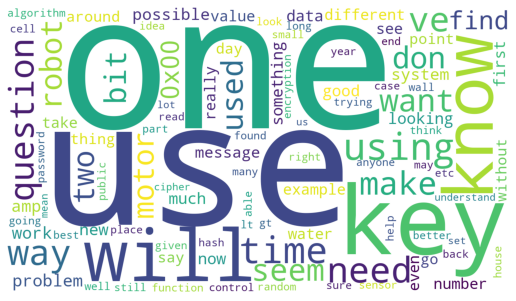
\includegraphics[scale=0.50]{figs/wordcloud1.png}
    \caption{Cluster de palavras}
    \label{fig:wordcloud1}
 \end{figure}

\section{Compressão de textos}
Os testes foram realizados com dois algoritmos clássicos de compressão \emph{sem perda} e suas versões baseadas em palavras (\textbf{Huffman}, \textbf{Huffword}, \textbf{LZ77}, \textbf{WLZ77}).
Neste conjunto de algoritmos estão presente algoritmos baseados em \emph{probabilidades associadas} e \emph{dicionários}
Os testes foram realizados sobre quatro algoritmos de compressão \textbf{sem perda} (apresentados no capítulo~\ref{cap:comp}), sendo dois baseados em \emph{caracteres} e os outros dois em \emph{palavras}
Uma hipótese razoável a ser validada é que com a versão baseada em palavras, o impacto da clusterização na taxa de compressão seja mais significativo.
A seguir, serão descritos alguns detalhes específicos da implementação dos compressores para o experimento (dando ênfase nos detalhes não contidos nos algoritmos em pseudocódigo apresentados no capítulo~\ref{cap:comp}).

\subsection{Classes auxiliares}
Para facilitar a reutilização de código na aplicação dos diferentes compressores, foi criada a classe auxiliar (\emph{TextCompressor}).
Nesta classe, são expostos os método \emph{encode(text)} e \emph{decode()} que servem como um ``contrato'' para a implementação dos algoritmos de compressão.
Cada classe que modela um compressor herda da classe base \emph{TextCompressor}, criando sua própria implementação dos métodos \emph{encode} e \emph{decode}.


\begin{lstlisting}[language=Python, caption=Classe TextCompressor]
class TextCompressor:
    def __init__(self):
        self.originaltext = None
        self.stats = None
    def encode(self, text):
        self.originaltext = text
        pass
    def decode(self):
        pass
\end{lstlisting}

Outra classe auxiliar implementada foi a \emph{CompressionStats}, uma interface para padronizar a leitura das métricas.

\begin{lstlisting}[language=Python, caption=Implementaçào da classe base CompressionStats]
class CompressionStats:
    def _avg_code(self):
        return (self.compressedtextsize / self.originaltextsize) * 8
    def _compression_rate(self):
        return 100 - (self.compressedtextsize / self.originaltextsize) * 100
    def __init__(self, originaltext, compressedtext):
        self.originaltextsize = len(originaltext)
        self.compressedtextsize = len(compressedtext)
    def __str__(self) -> str:
        return stats_text.format(csize=self._avg_code(), osize=self.originaltextsize, nsize=self.compressedtextsize, crate=self._compression_rate())
\end{lstlisting}

\subsection{Compressão baseada em palavras}
Para a implementação dos algoritmos baseados em \textbf{palavras}, boa parte do código fonte utilizado nos algoritmos ``canônicos'' foram reutilizados.
Como o \emph{Python} é uma linguagem de \textbf{tipagem dinâmica}, a implementação ``canônica'' interpreta a entrada como um vetor de \emph{símbolos} (sem necessariamente distinguir o tipo de símbolo).
Com isso, podemos reaproveitar grande parte das funções escritas independente do alfabeto de origem utilizado. 

O \emph{Huffword} computa as \emph{palavras} e \emph{separadores} como duas entradas distintas.
Para dividir a entrada entre \emph{palavras} e \emph{separadores}, foi utilizada a biblioteca \emph{re}, que permite executar buscas em \emph{strings} utilizando \emph{regex}.
A mesma lógica é aplicada ao \emph{WLZ77}, diferindo do fato que desta vez, as \emph{palavras} e \emph{separadores} são processadas em um único vetor.

\begin{lstlisting}[language=Python, caption=Função \emph{encode} para o \emph{Huffword}]
def _build_huffword_code(seq):
    freqs = frequency_dictionary(seq)
    huff_tree = canonical.build_huff_tree(freqs)
    code_table= canonical.build_code_table(huff_tree)
    return code_table
    
def huffword_encode(text):
    # Words huff tree
    words = re.findall(r'\w+', text)
    words_code = _build_huffword_code(words)

    # Non words huff tree
    nonwords = re.findall(r'\W+', text)
    nonwords_code = _build_huffword_code(nonwords)

    encoded_string = ""

    # When text start with non-word append 0, otherwise append 1
    starts_with = 0
    if text.startswith(words[0]):
        starts_with += 1
    
    # Append starts with as the first char
    encoded_string += str(starts_with)

    # Encode intercalating words and nonwords
    w_index = 0
    nw_index = 0

    #When starts with non words
    if not starts_with:
        encoded_string += nonwords_code[nonwords[0]]
    
    while w_index < len(words) or nw_index < len(nonwords):
        if w_index < len(words):
            word = words[w_index]
            encoded_string += words_code[word]
            w_index += 1
        
        if nw_index < len(nonwords):
            nonword = nonwords[nw_index]
            encoded_string += nonwords_code[nonword]
            nw_index += 1
    
    return {'encoded' : encoded_string,
            'words_meta' : (words, words_code),
            'non_words_meta': (nonwords, nonwords_code)}
\end{lstlisting}



\section{Partição de dados}
Os testes com os algoritmos de compressão foram realizados com duas estratégias diferentes de partição.
Na primeira, os dados são particionados \textbf{aleatoriamente} em $n$ partes.
Já para o teste com a clusterização, os mesmos dados são particionados em $n$ \emph{clusters} criados pelo algoritmo \emph{k-means}.
Em ambos os casos, cada algoritmo de compressão foi executado sobre as $n$ partições (grupos) e as métricas foram computadas por média média aritmética simples.

\subsection{Partição aleatória} \label{ssec:randomp}
Para o teste com partição aleatória, o \emph{dataframe} original foi dividido em $n$ partes iguais.
É importante que tais divisões sejam aleatórias, a fim de evitar possíveis ruídos no teste.

Para garantir a aleatoriedade, foi utilizado o método $.sample()$ da biblioteca $pandas$. 
Este método cria uma amostra aleatória de itens para um determinado eixo do objeto. 
O parâmetro $frac=1$ faz com que o método retorne uma amostra com todos os dados originais (porém de maneira randômica).
Em seguida, o vetor foi fracionado pela função $array\_split()$ da biblioteca $numpy$.

\begin{lstlisting}[language=Python, caption=Partição aleatória de dados]
# Data to compress: Compress the original data raw
raw_text = df['content']

#Shuffle raw text
shuffle = raw_text.sample(frac=1)
partitions = np.array_split(shuffle, n_partitions)
\end{lstlisting}

\subsection{Clusterização}
Para o teste com partição por clusterização, o algoritmo \emph{k-means} foi utilizado.
A clusterização se inicia transformando os dados textuais em \textbf{vetores de características}, utilizando a técnica de vetorização \emph{TF-IDF}. 
O vetor de características passa por uma redução de dimensionalidade via \emph{PCA} (reduzindo os dados em \textbf{duas} componentes principais, para melhor visualização).

\begin{lstlisting}[language=Python, caption=Vetorização dos dados]
def identity_tokenizer(text):
  return text

vect = TfidfVectorizer(tokenizer=identity_tokenizer,lowercase=False)
tf_idf = vect.fit_transform(df['sanitezed_content'].values)
tf_idf_norm = normalize(tf_idf) # To PCA running
tf_idf_arr = tf_idf_norm.toarray()
p.DataFrame(tf_idf_arr, columns=vect.get_feature_names()).head(10)

# PCA component reduction
pca = PCA(n_components=2)
Y = pca.fit_transform(tf_idf_arr)
\end{lstlisting}

Com os dados vetorizados em duas dimensões, o \emph{método de elbow} é utilizado para encontrar o número ``ideal'' de clusters.
O gráfico de elbow foi construído com os número de clusters variando entre 1 e 7. 
De acordo com os resultados obtidos, foi utilizado $n=3$ como parâmetro para o \emph{k-means}.

 \begin{figure}[H]
   \centering
   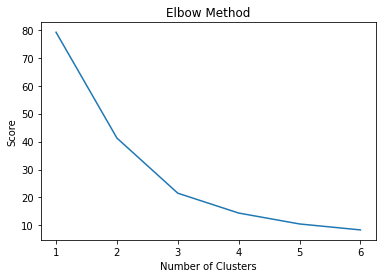
\includegraphics[scale=0.75]{figs/elbowgraph.png}
    \caption{Método de Elbow}
    \label{fig:melbow}
 \end{figure}

Por fim, o \emph{k-means} é aplicado a base de dados através do objeto $sklearn.cluster.KMeans$.
O parâmetro $n\_clusters$ recebe o número de clusters encontrado no passo anterior. 
O parâmetro $init$ indica a utilização do \emph{k-means++} na inicialização dos pontos centrais.
Já o parâmetro  $max\_inter$, define como 50 o número máximo de iterações do algoritmo \emph{k-means}.

\begin{lstlisting}[language=Python, caption=Vetorização dos dados]
kmeans = KMeans(n_clusters=n_clusters, init='k-means++', max_iter=50)
fit_data = kmeans.fit(Y)
pred_class = kmeans.predict(Y)

display(fit_data.labels_)
df['Cluster'] = fit_data.labels_
\end{lstlisting}

 \begin{figure}[H]
   \centering
   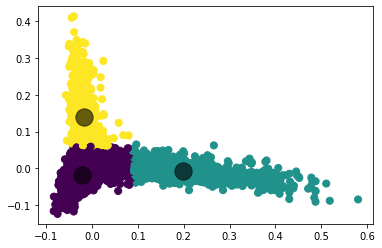
\includegraphics[scale=0.85]{figs/clustercloud.png}
    \caption{Distribuição dos clusters (dados vetorizados)}
    \label{fig:clustercloud}
 \end{figure}

\section{Resultados}
\subsection{Taxa de compressão}
Para validar a hipótese inicial, os dados particionados (aleatoriamente ou via compressão) foram comprimidos utilizando os algoritmos citados anteriormente.
Cada partição foi processada de maneira \textbf{individual}, portanto, a performance geral de cada algoritmo foi obtida a partir da média aritmética entre os resultados das $n$ partições.

Para compressão de dados sem perda o objetivo é reduzir o tamanho da mensagem, sem haver perda de informações.
Assim, uma das principais métricas de sucesso nestes algoritmos é a \textbf{taxa de compressão}.
Definimos a \textbf{taxa de compressão} como a razão entre o tamanho do documento codificado e o original.

\begin{equation}\label{eq:tf}
taxa~de~compressão = \frac{tamanho~do~documento~codificado}{tamanho~do~documento~original}
\end{equation}\label{eq:tf}

Definimos $\Delta$ como o impacto da clusterização na taxa de compressão, que é obtido pela diferença entre os resultados com e sem a clusterização.
 \begin{figure}[H]
   \centering
   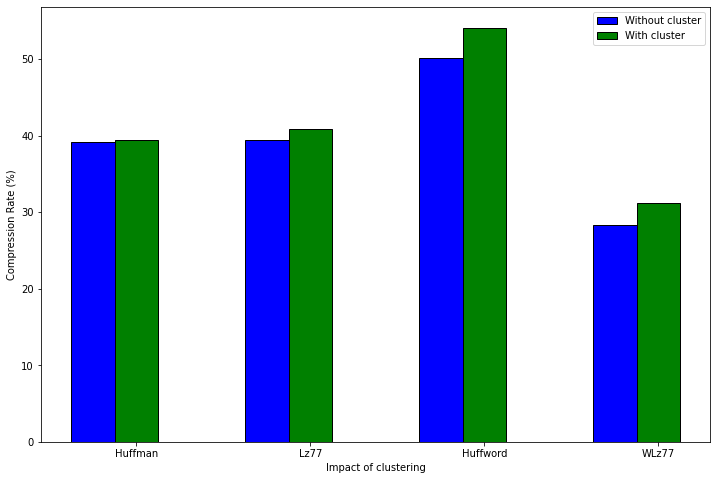
\includegraphics[scale=0.60]{figs/graphfinal.png}
    \caption{Impacto da clusterização na taxa de compressão}
    \label{fig:clusterfinalgraph}
 \end{figure}
 
 \begin{table}[H]
   \centering
   \caption{Impacto da clusterização na taxa de compressão} \label{tab:resultcomp}
   \begin{tabular}{|l|c|c|c|c|c|c|r|}
        \hline
        \small{Algoritmo} & \small{\% compressão} &  \small{\% compressão (clusters)} & \small{$\Delta$} \\ \hline
              Huffman   &   39.214536 & 39.395034 & 0.180498 \\ \hline
              Huffword  &   50.133603 & 54.096327 & 3.962724 \\ \hline
              LZ77        &   39.470517 & 40.795727 & 1.325210 \\ \hline
              WLZ77    &   28.369986 & 31.173907 & 2.803921 \\ \hline
  \end{tabular}
\end{table}

Conforme previsto no capítulo~\ref{cap:comp}, a tabela~\ref{tab:resultcomp} mostra que a clusterização teve um maior impacto nos algoritmos baseados em \textbf{palavras}.
Em especial, o maior $\Delta$ foi alcançado para o \emph{Huffword},com uma melhoria de \textbf{quase 4\%}. Curiosamente, a versão baseada em palavras do LZ77 se mostrou menos efetiva no geral do que sua versão canônica.

\subsection{Tempo de execução}
Outra métrica que auxilia na comparação entre os algoritmos é o \textbf{tempo de execução}.
Para isso, foi utilizado o comando \emph{\%time\%} do \emph{jupyter notebook} (que mede o tempo de execução da célula em que o comando foi inserido).

\begin{table}[H]
   \centering
   \caption{Tempo de execução dos algoritmos de compressão} \label{tab:vcode}
   \begin{tabular}{|l|c|c|c|c|c|c|r|}
        \hline
        \small{Algoritmo} & \small{Tempo de execução} & \small{Partição} \\ \hline
              Huffman   &   2.18s                        & aleatória \\ \hline
              Huffword  &   2.8s                          & aleatória \\ \hline
              LZ77        &   8min 24s                  & aleatória \\ \hline
              WLZ77    &   1h 37min 41s           & aleatória \\ \hline
              Huffman  &   3.08s                       & k-means \\ \hline
              Huffword &   3.66s                       & k-means \\ \hline
              LZ77       &   12min 24s               & k-means \\ \hline
              WLZ77   &   2h 30min 9s            & k-means \\ \hline
  \end{tabular}
\end{table}

Fica claro que as versões baseadas em palavras e clusterizadas via \emph{k-means} consomem mais tempo de execução.
Este dado já era esperado, já que o aumento de símbolos semelhantes leva a mais \emph{tokenizações} e por consequência maior tempo de processamento.

\section{Conclusão}
Neste trabalho, combinamos o uso da compressão \textbf{baseada} em palavras com a clusterização, em busca de uma melhora na taxa de compressão para base textuais.
Os resultados experimentais confirmam as hipóteses levantadas previamente, 
e chega-se à conclusão de que a clusterização impacta \textbf{positivamente} a \textbf{taxa de compressão} de textos.
Entretanto, os experimentos também mostraram um aumento nos recursos consumidos (tanto pelo pré-processamento, quanto pela compressão em si).
Espera-se que os resultados apresentados neste trabalho sejam úteis na implementação de ferramentas de compressão otimizadas, principalmente para grandes bases de dados textuais.

\section{Trabalhos futuros}
O intuito principal deste trabalho era apresentar a clusterização como potencializador para alguns algoritmos clássicos de compressão sem perda.
Algoritmos mais modernos (como BZip e WBW), otimizados especificamente para grandes textos, podem trazer resultados ainda melhores com a compressão.
Utilizar outros métodos de clusterização mais complexos (como a clusterização hierárquica), também podem trazer resultados diferentes para os testes.
